\documentclass[12pt,letterpaper]{article}
\usepackage{fullpage}
\usepackage[top=2cm, bottom=4.5cm, left=2.5cm, right=2.5cm]{geometry}
\usepackage{amsmath,amsthm,amsfonts,amssymb,amscd}
\usepackage{lastpage}
\usepackage{enumerate,enumitem}
\usepackage{fancyhdr}
\usepackage{mathrsfs}
\usepackage{xcolor}
\usepackage{graphicx}
\usepackage{listings}
\usepackage{hyperref}
\usepackage{listings}
\usepackage{tikz}
\usepackage{braket}
\usepackage{graphicx}
\usetikzlibrary{shapes}

\usepackage[edges]{forest}

\hypersetup{%
  colorlinks=true,
  linkcolor=blue,
  linkbordercolor={0 0 1}
}
 
\renewcommand\lstlistingname{Algorithm}
\renewcommand\lstlistlistingname{Algorithms}
\def\lstlistingautorefname{Alg.}

\lstdefinestyle{Python}{
    language        = Python,
    frame           = lines, 
    basicstyle      = \footnotesize,
    keywordstyle    = \color{blue},
    stringstyle     = \color{green},
    commentstyle    = \color{red}\ttfamily
}

\setlength{\parindent}{0.0in}
\setlength{\parskip}{0.05in}

% Edit these as appropriate
\newcommand\course{NLP (0368307701)}
\newcommand\institute{Tel Aviv University}
\newcommand\hwnumber{1}
\newcommand\ID{Morris Alper, Pavel Rastopchin}

\pagestyle{fancyplain}
\headheight 35pt
\lhead{\ID \\ \institute}
\chead{\textbf{\Large Homework \hwnumber}}
\rhead{\course \\ \today}
\lfoot{}
\cfoot{}
\rfoot{\small\thepage}
\headsep 1.5em

\begin{document}

\section*{Section 1 - Preliminaries}

(empty)

\section*{Section 2 - Understanding word2Vec}

\begin{itemize}
    \item[(a)] Write the elements of the vector as $\mathbf{x} = (x_i)_i$. Then
    $$\text{softmax}(\mathbf{x} + c) = \left(\frac{e^{x_i + c}}{\sum_j e^{x_j + c}}\right)_i = \left(\frac{e^c e^{x_i}}{e^c \sum_j e^{x_j}}\right)_i = \left(\frac{e^{x_i}}{\sum_j e^{x_j}}\right)_i = \text{softmax}(\mathbf{x})$$
    \item[(b)]
    $y_w$ is $1$ for $w=o$ and $0$ otherwise, so
    
    $$- \sum_{w \in W}y_w \log(\hat{y}_w) = - y_o \log(\hat{y}_o) - \sum_{w \in W, w \neq o}y_w \log(\hat{y}_w) = - 1 \cdot \log(\hat{y}_o) - \sum_{w \in W, w \neq o}0 \cdot \log(\hat{y}_w) = - \log(\hat{y}_o)$$
    \item[(c)]
    
    $$\frac{\partial \mathbf{J}_{naive-softmax}}{\partial \mathbf{v}_c} = - \frac{\partial}{\partial \mathbf{v}_c} \log \frac{e^{\mathbf{u}_o^T \mathbf{v}_c}}{\sum_{w \in W} e^{\mathbf{u}_w^T \mathbf{v}_c}}$$
    $$= - \frac{\partial}{\partial \mathbf{v}_c} \left( \mathbf{u}_o^T \mathbf{v}_c - \log \sum_{w \in W} 
    e^{\mathbf{u}_w^T \mathbf{v}_c} \right)$$
    $$= - \mathbf{u}_o + \left(\sum_{w \in W} \mathbf{u}_w e^{\mathbf{u}_w^T \mathbf{v}_c} \right) \left( \sum_{w \in W} 
    e^{\mathbf{u}_w^T \mathbf{v}_c} \right)^{-1}$$
    $$= - \mathbf{u}_o + \sum_{w \in W} \text{softmax}_w(\mathbf{u}_w^T \mathbf{v}_c) \mathbf{u}_w $$
    $$=\sum_{w \in W} (\text{softmax}_w(\mathbf{u}_w^T \mathbf{v}_c) - \delta_{o, w}) \mathbf{u}_w $$
    
    Where $\delta_{o,w}$ equals $1$ if $o = w$ and $0$ otherwise.
    
    \item[(d)]
    
    $$\frac{\partial \mathbf{J}_{naive-softmax}}{\partial \mathbf{u}_w} = - \frac{\partial}{\partial \mathbf{u}_w} \log \frac{e^{\mathbf{u}_o^T \mathbf{v}_c}}{\sum_{w' \in W} e^{\mathbf{u}_{w'}^T \mathbf{v}_c}}$$
    $$= - \frac{\partial}{\partial \mathbf{u}_w} \left( \mathbf{u}_o^T \mathbf{v}_c - \log \sum_{w' \in W} e^{\mathbf{u}_{w'}^T \mathbf{v}_c} \right)$$
    $$= -\delta_{o,w}\mathbf{v}_c + \mathbf{v}_c e^{\mathbf{u}_w^T \mathbf{v}_c} \left( \sum_{w' \in W} e^{\mathbf{u}_{w'}^T \mathbf{v}_c} \right)^{-1}$$
    $$= (\text{softmax}_w(\mathbf{u}_w^T \mathbf{v}_c)-\delta_{o,w})\mathbf{v}_c$$
    
    Where $\delta_{o,w}$ equals $1$ if $o = w$ and $0$ otherwise. This gives the solution in both cases ($w=o$ and $w \neq o$).
    
    \item[(e)]
    The $i$-th element of $\sigma(\mathbf{x})$ is $\sigma(x_i) = (1+e^{-x_i})^{-1}$, so
    
    $$\frac{d \sigma(x_i)}{d x_i} = e^{-x_i}(1 + e^{-x_i})^{-2} = e^{-x_i}(\sigma(x_i))^2 = ((\sigma(x_i))^{-1}-1)(\sigma(x_i))^2 = \sigma(x_i)(1 - \sigma(x_i))$$
    
    Since this holds for each element of $\sigma(\mathbf{x})$, we can express the vector-valued derivative as
    
    $$\frac{d \sigma(\mathbf{x})}{d \mathbf{x}} = \sigma(\mathbf{x})^T(1 - \sigma(\mathbf{x}))$$
    
    
    \item[(f)]
    
    Note that in general $\frac{d}{dx} \log \sigma(x) = \sigma(x)(1-\sigma(x))(\sigma(x))^{-1} = 1 - \sigma(x) = \sigma(-x)$. We will use this in the following calculations.
    
     $$\frac{\partial \mathbf{J}_{neg-sample}}{\partial \mathbf{v}_c} = - \frac{\partial}{\partial \mathbf{v}_c} \log \sigma(\mathbf{u}_o^T\mathbf{v}_c) - \sum_{k=1}^K \frac{\partial}{\partial \mathbf{v}_c} \log \sigma(-\mathbf{u}_k^T\mathbf{v}_c)$$
     $$= - \mathbf{u}_o (1-\sigma(\mathbf{u}_o^T \mathbf{v}_c)) - \sum_{k=1}^K (-\mathbf{u}_k)(1- \sigma(-\mathbf{u}_k^T\mathbf{v}_c))$$
     $$= -\sigma(-\mathbf{u}_o^T \mathbf{v}_c)\mathbf{u}_o + \sum_{k=1}^K \sigma(\mathbf{u}_k^T\mathbf{v}_c) \mathbf{u}_k$$
     
     $$\frac{\partial \mathbf{J}_{neg-sample}}{\partial \mathbf{u}_o} = - \frac{\partial}{\partial \mathbf{u}_o} \log \sigma(\mathbf{u}_o^T\mathbf{v}_c) - \sum_{k=1}^K \frac{\partial}{\partial \mathbf{u}_o} \log \sigma(-\mathbf{u}_k^T\mathbf{v}_c)$$
     $$= - \mathbf{v}_c (1 - \sigma(\mathbf{u}_o^T\mathbf{v}_c)) - 0$$
     $$= -\sigma(-\mathbf{u}_o^T\mathbf{v}_c) \mathbf{v}_c$$
     
     $$\frac{\partial \mathbf{J}_{neg-sample}}{\partial \mathbf{u}_k} = - \frac{\partial}{\partial \mathbf{u}_k} \log \sigma(\mathbf{u}_o^T\mathbf{v}_c) - \sum_{k'=1}^K \frac{\partial}{\partial \mathbf{u}_{k'}} \log \sigma(-\mathbf{u}_k^T\mathbf{v}_c)$$
     $$= - 0 - \frac{\partial}{\partial \mathbf{u}_k} \log \sigma(-\mathbf{u}_k^T\mathbf{v}_c)$$
     $$= -(-\mathbf{v}_c)(1-\sigma(-\mathbf{u}_k^T\mathbf{v}_c))$$
     $$= \sigma(\mathbf{u}_k^T\mathbf{v}_c)\mathbf{v}_c$$
    
    This loss function is more efficient to compute than the naive softmax loss because it requires computing only $K+1$ vector dot products, while the naive softmax loss requires calculating $\left|W\right| + 1$ vector dot products, where $\left|W\right|$ is the number of words in the vocabulary. (The same is true for the gradients of the losses; the gradients of the naive softmax loss calculate a softmax over all $\left|W\right|$ words, while each gradient of the negative sampling loss each require at most $K+1$ dot products to be calculated.)
    
    \item[(g)]
    
        $$\frac{\partial \mathbf{J}_{skip-gram}}{\partial \mathbf{U}}(\mathbf{v}_c, w_{t-m}, \ldots, w_{t+m}, \mathbf{U}) = \sum_{-m \leq j \leq m, j \neq 0}\frac{\partial \mathbf{J}}{\partial \mathbf{U}}(\mathbf{v}_c, w_{t+j}, \mathbf{U})$$
        
        $$\frac{\partial \mathbf{J}_{skip-gram}}{\partial \mathbf{v}_c}(\mathbf{v}_c, w_{t-m}, \ldots, w_{t+m}, \mathbf{U}) = \sum_{-m \leq j \leq m, j \neq 0}\frac{\partial \mathbf{J}}{\partial \mathbf{v}_c}(\mathbf{v}_c, w_{t+j}, \mathbf{U})$$
        
        And for $w \neq c$:
        
        $$\frac{\partial \mathbf{J}_{skip-gram}}{\partial \mathbf{v}_w}(\mathbf{v}_c, w_{t-m}, \ldots, w_{t+m}, \mathbf{U}) = 0$$
    
    
\end{itemize}

\section*{Section 3 - Implementing word2Vec}

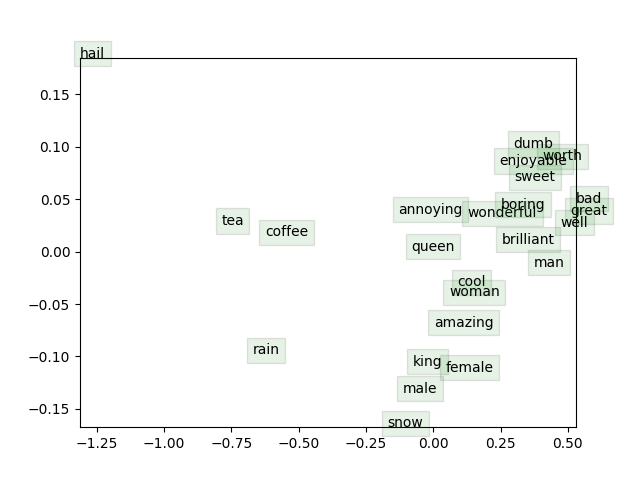
\includegraphics{word_vectors.png}

We see some logical clusters of words, for example: "tea" and "coffee" are close to each other, as are "queen" and "woman", "king" and "male". All of the descriptive adjectives seem to cluster to the right.

On the other hand, "rain" and "hail" are far apart, and we cannot clearly see word analogies of the form "king:queen as male:female".

These results could perhaps be improved by training on a larger dataset and/or modifying the training regime (e.g. modifying regularization, early stopping heuristics, etc.). Also, the low embedding dimensionality could be the cause. However it is also possible that we are just limited by our 2-D visualization, which may not display all clusters of word embeddings clearly as data is lost in the dimensionality reduction.

\section*{Section 4 - Optimizing word2Vec}

\begin{itemize}
    \item[(a)]
    Let $V = \{v_1, v_2, \cdots, v_k\}$ be the vocabulary, containing $k$ words. Then $\theta$ may be modeled as a $k \times k$ matrix whose $i,j$-th element $\theta_{i,j}$ is equal to $p_\theta(v_j | v_i)$ (probability that word $v_j$ co-occurs with $v_i$ (within window of width $m$).
    
    Simplify the (log-)objective as follows, by grouping together terms in the initial sum for the same word occuring multiple times in the corpus:
    
    $$J(\theta) = \sum_{t=1}^T \sum_{-m \leq j \leq m} \log p_\theta (w_{t+j} | w_t) = \sum_{i=1}^k \sum_{j=1}^k  \#(v_i, v_j) \log p_\theta (v_j | v_i)$$
    $$= \sum_{i=1}^k \sum_{j=1}^k  \#(v_i, v_j) \log \theta_{i, j} = \sum_{i=1}^k J_i(\theta)$$
    
    where we define $J_i(\theta) = \sum_{j=1}^k  \#(v_i, v_j) \log \theta_{i, j}$.
    
    We want to find $\theta^* = \arg \max_\theta J(\theta)$. We may fix $i$ and find $\theta_{i,1}, \theta_{i,2}, \ldots, \theta_{i, k}$ that maximize $J_i(\theta)$, since only the $J_i$ term in $J$ depends on these parameters.
    
    The parameters have the constraints $0 \leq \theta_{i, j} \leq 1$ and $\sum_k \theta_{i, k} = 1$ for all $j \in \{1, 2, \ldots, k\}$. So we can find the arg max by using the method of Lagrange multipliers:
    
    $$\text{objective function: } F_i(\theta) = \sum_{j=1}^k \#(v_i, v_j) \log \theta_{i,j}$$
    $$\text{constraint function: } G_i(\theta) = \sum_k \theta_{i, k} - 1$$
    
    $$\mathcal{L}_i(\theta, \lambda) = F_i(\theta) - \lambda G_i(\theta)$$
    
    $$\frac{\mathcal{L}_i}{\theta_{i, j}} = \frac{\#(v_i, v_j)}{\theta_{i, j}} - \lambda$$
    
    So $\nabla \mathcal{L}_i(\theta^*, \lambda^*) = 0$ implies that $\frac{\#(v_i, v_j)}{\theta^*_{i,j}} - \lambda^* = 0$ for all $i, j = 1, \ldots, k$, and therefore $$\theta^*_{i, j} = \frac{\#(v_i, v_j)}{\lambda^*}$$.
    
    Since $\sum_{j=1}^k \theta_{i, j} = 1$, it follows that $\lambda^* = \sum_{j=1}^k \#(v_i, v_j)$, so
    
    $$\theta^*_{i, j} = \frac{\#(v_i, v_j)}{\sum_{j=1}^k \#(v_i, v_j)}$$
    
    These values of $\theta^*_{i, j}$ are thus are the unique critical point for $\mathcal{L}_i$ under the constraints. Since the Hessian matrix $H(\mathcal{L}_i)$ is diagonal with diagonal elements $-\frac{\#(v_i, v_j)}{\theta_{i,j}^2} < 0$, $H(\mathcal{L}_i)$ is negative definite (in general, and specifically at $\theta^*$) so the critical point is a maximum.
    
    Therefore $\theta^*$ is the arg max of $J$, and so by definition $p_{\theta^*}(v_j | v_i) = \theta^*_{i,j} = \frac{\#(v_i, v_j)}{\sum_{j=1}^k \#(v_i, v_j)}$, proving the claim in the question. 
    
    \item[(b)]
    
    We represent the four words as the characters ``a", ``b", ``c", ``d', and consider the corpus consisting of four sentences ``aa", ``bb", ``cc", and ``dd".
    
    The optimum solution from part (a) gives $p(x|x) = 1$ and $p(y|x) = 0$ for $x \neq y$ (e.g. $p(a|a)=1$, $p(c|b) = 0$, etc.).
    
    Word2vec assigns to each word $w$ two word embedding vectors $u_w$ and $v_w$. For this question we assume that these are of dimension one - i.e. scalars. So we have eight scalars: $u_a, v_a, u_b, v_b, u_c, v_c, u_d, v_d$.
    
    Word2vec models the probability of word co-occurence as
    
    $$p(y | x) = \text{softmax}_o(u_y^T v_x) = \text{softmax}_y(u_y v_x) = \frac{e^{u_y v_x}}{\sum_i e^{u_{y_i} v_x}}$$
    
    where we removed the transpose since each $u$ and $v$ are scalars in our case.
    
    For the optimal solution, $p(y|x)=0$ when $x \neq y$, but the softmax above will always take a positive value since all the exponential terms are positive. Therefore there is no assignment of scalars $u_\cdot, v_\cdot$ that give the optimal solution.
    
    
    
    
    
    
\end{itemize}

\section*{Section 5 - Paraphrase Detection}

\begin{itemize}
    \item[(a)]
    
    Since $\text{relu}(\mathbf{x_1})$ and $\text{relu}(\mathbf{x_2})$ only have non-negative terms, $\text{relu}(\mathbf{x_1})^T \text{relu}(\mathbf{x_2}) \geq 0$, so the input to $\sigma$ will always be non-negative and thus $\sigma$ will always return at least $0.5$ and the binary classifier will return label $1$ (positive, paraphrase). Since the dataset contains $3$ negative examples for every $1$ positive example, this classifier which always outputs $1$ will have accuracy $1/4=0.25$.
    
    \item[(b)]
    
    This can be corrected for by adding a (negative) bias term in the sigmoid
    $$\sigma(\text{relu}(\mathbf{x_1})^T \text{relu}(\mathbf{x_2}) + b)$$
\end{itemize}

\end{document}
